RGG allows you to provide paths to MeshKit\footnote{See \url{http://trac.mcs.anl.gov/projects/fathom/wiki/MeshKit}.} and Cubit\footnote{See \url{https://cubit.sandia.gov/}.} executables to facillitate the production of meshes for simulation.

\section{Add Paths to Preferences}

Access the \emph{system preferences window} by clicking on the \emph{edit menu} of the \emph{toolbar}.

\begin{figure}[H]
	\begin{center}
		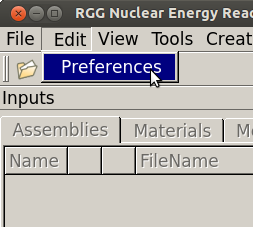
\includegraphics[width=0.5\linewidth]{Images/mesh-1.png}
		\caption{Opening RGG preferences.}
		\label{fig:Mesh1}
	\end{center}
\end{figure}

This brings up the system preferences window.  To add AssyGen, CoreGen, or Cubit, click the \emph{browse button} to locate the executable and click the \emph{open button} to get back to the system preferences window.

\begin{figure}[H]
	\begin{center}
		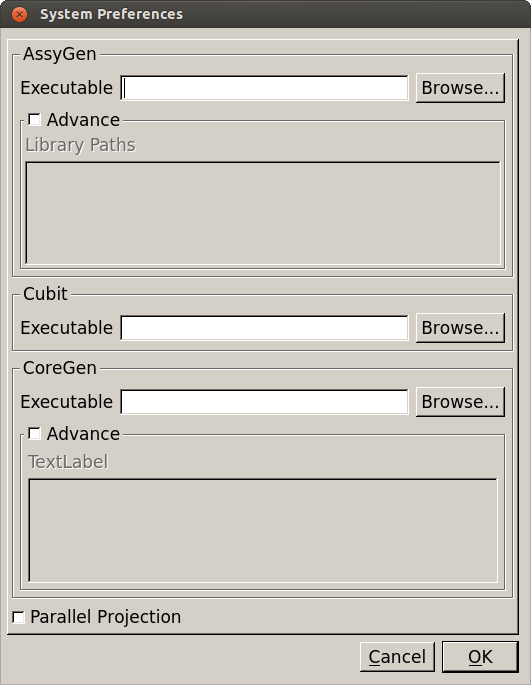
\includegraphics[width=0.5\linewidth]{Images/mesh-2.png}
		\caption{The preferences window.}
		\label{fig:Mesh2}
	\end{center}
\end{figure}